%!TeX root=../document.tex

\chapter{Static Solution}

Having assembled the various element equations into an overall equation of motion for the bow-and-arrow system, the actual simulation consists of solving these equations of motion for a given initial state and boundary conditions.
Different numerical methods are used for this, depending on whether a static or dynamic analysis is to be performed.

The first part of the bow simulation, which encompasses the bracing of the bow and drawing it from brace height to full draw, is static in nature.
That's because the process is fairly slow and therefore the influence of the moving masses of the bow can be neglected.
A System as ours, with an equation of motion of the form

\begin{equation}
\boldsymbol{M}\ddot{\boldsymbol{u}} + \boldsymbol{Q}(\boldsymbol{u},\,\dot{\boldsymbol{u}}) = \boldsymbol{P},
\end{equation}

is in static equilibrium if the nodal positions~$\boldsymbol{u}(t)$ stay constant over time.
This requires the velocities and accelerations to be zero, i.e.~$\dot{\boldsymbol{u}}(t),\,\ddot{\boldsymbol{u}}(t) \equiv \boldsymbol{0}$, leading to the static equilibrium condition

\begin{equation}
\underbrace{\boldsymbol{Q}(\boldsymbol{u},\,\boldsymbol{0}) - \boldsymbol{P}}_{\boldsymbol{R}(\boldsymbol{u})} = \boldsymbol{0}. \label{eq:statics:equilibrium}
\end{equation}

Put into words, all components of the internal forces~$\boldsymbol{Q}$ have to be in balance with the respective external loads~$\boldsymbol{P}$.
We introduce the residual forces~$\boldsymbol{R}(\boldsymbol{u})$ as a shorthand for the difference between both.
The equilibrium condition~$\boldsymbol{R}(\boldsymbol{u}) = \boldsymbol{0}$ is a nonlinear system of equations for the unknown equilibrium displacements~$\boldsymbol{u}$ and/or external forces~$\boldsymbol{P}$, depending on the exact problem statement.

\section{The Basic Newton-Raphson Method}

In the most basic case, the external loads are given and the task is to calculate the corresponding equilibrium displacements.
Equation~(\ref{eq:statics:equilibrium}) then becomes a nonlinear system of equations in $\boldsymbol{u}$.
Solving it can only be done numerically except for very simple systems.
An often used method for this kind of problem is the Newton-Raphson method. The basic idea behind it is to linearize the equilibrium equation~(\ref{eq:statics:equilibrium}) around a known displacement vector~$\boldsymbol{u}_i$ and solve the resulting linear equation in order to obtain an improved approximation~$\boldsymbol{u}_{i+1}$.
Starting with an initial value~$\boldsymbol{u}_0$, the procedure is repeated until the solution is accurate enough by some convergence criterion.
Lineraization of (\ref{eq:statics:equilibrium}) yields

\begin{align}
\boldsymbol{R}(\boldsymbol{u}_i) +
\underbrace{
\left(\frac{\partial \boldsymbol{R}}{\partial \boldsymbol{u}}\bigg \vert_{\boldsymbol{u}_i}\right)
}_{\boldsymbol{K}(\boldsymbol{u}_i)}
\underbrace{
(\boldsymbol{u}_{i+1} - \boldsymbol{u}_i)
}_{\Delta\boldsymbol{u}_i} &= \boldsymbol{0}
\end{align}

Solving this for the solution increment~$\Delta\boldsymbol{u}_i$ leads to the iterative procedure

\begin{align}
\Delta\boldsymbol{u}_i &= \boldsymbol{K}^{-1}(\boldsymbol{u}_i)\left(\boldsymbol{P} - \boldsymbol{Q}(\boldsymbol{u}_i)\right),\label{eq:statics:newton_linear_solution}\\
\boldsymbol{u}_{i+1} &= \boldsymbol{u}_i + \Delta\boldsymbol{u}_i.\label{eq:statics:newton_iteration}
\end{align}

which is carried out until the solution is accurate enough, as determined by a convergence criterion based on either the increment~$\Delta\boldsymbol{u}_i$, the residual~$\boldsymbol{R}(\boldsymbol{u}_i)$ or a combination of both.
We will have a more thorough look at the convergence criterion later.
In the implementation, the tangent stiffness matrix in~\eqref{eq:statics:newton_linear_solution} is not actually inverted, because that would be numerically inefficient.
Instead,~$\Delta\boldsymbol{u}_i$ is obtained by solving the equivalent linear system of equations using an appropriate matrix decomposition.
Since the tangent stiffness matrix is symmetric, an algorithm that exploits this can be selected.
It is not generally positive definite though, unlike the stiffness matrices of many linear mechanical systems.

This basic Newton-Raphson scheme can be improved and extended in many ways, for example by combining it with a line search or by avoiding the calculation of the tangent stiffness matrix at every iteration.
Some keywords in this respect are \textit{simplified Newton methods} and \textit{quasi-Newton methods} such as the \textit{BFGS method}.
The first extension we are going to look at, which is essential for our bow simulation, is \textit{displacement control}.

\newpage
\section{Load- and Displacement Control}
\label{sec:constrained-newton-raphson}

When simulating the drawing of the bow, the set of known and unknown variables is not quite as assumed in the previous section.
The vector of external forces consists of the draw force, which is applied at the center node of the string.
But while the direction of this draw force is known, its magnitude is not.
We only know the position of the string node, since that corresponds to the current draw length at which the bow is to be evaluated.
A solution to this is displacement control, where we prescribe a value for one of the displacement components and instead treat the magnitude of the external forces as a variable that is determined during solution.
Displacement control also has the additional benefit that it still works when there is a decrease of load in the force-draw curve, which can theoretically happen with some extreme recurve designs.

Before the bow is being drawn, there is actually another static simulation step: bracing.
Starting from the bow's initial, unbraced state, the braced equilibrium state of the bow with an applied string is determined.
The bracing simulation is described in more detail later, but it also makes use of displacement control.

The following derivations have been adapted from \cite{bib:kuhl2002}. Displacement control is a special case of a wider class of methods where the equilibrium equations are modified as

\begin{align}
\boldsymbol{Q}(\boldsymbol{u}) - \lambda\,\boldsymbol{P} &= 0,\label{eq:equilibrium_dc}\\
c(\boldsymbol{u},\,\lambda) &= 0.\label{eq:constraint_dc}
\end{align}

Here the external forces are scaled by the unknown load factor~$\lambda$. To compensate for this additional unknown, a scalar constraint~$c(\boldsymbol{u},\,\lambda) = 0$ on the displacements and the load parameter is introduced.
Depending on the choice of constraint the method can be turned into load control, displacement control or other more sophisticated schemes like the arc-length method. We will carry out the derivation for the general case and specify the constraints later.
Let us first restate equations~(\ref{eq:equilibrium_dc}) and~(\ref{eq:constraint_dc}) in more general terms as
%
\begin{align}
\boldsymbol{f}(\boldsymbol{x},\,\lambda) &= \boldsymbol{0}, \label{eq:equilibrium_dc_gen} \\
c(\boldsymbol{x},\,\lambda) &= 0, \label{eq:constraint_dc_gen}
\end{align}

with the functions~$\boldsymbol{f}: \mathbb{R}^n,\,\mathbb{R} \rightarrow \mathbb{R}^n$ and~$c: \mathbb{R}^n,\,\mathbb{R} \rightarrow \mathbb{R}$.
This system of nonlinear equations has to be solved for the unknown vector~$\boldsymbol{x}$ and the scalar parameter~$\lambda$.
Like before, the Newton-Raphson method is used: The equations are linearized around a given approximation~$\{\boldsymbol{x}_i,\,\lambda_i\}$ and the resulting linear system is solved to obtain an improved approximiation~$\{\boldsymbol{x}_{i+1},\,\lambda_{i+1}\}$.
This process is repeated iteratively until~$\boldsymbol{x}$ and~$\lambda$ satisfy both the vector equation as well as the scalar constraint reasonably well as determined by some convergence criterion.
Carrying out the linearization leads to the two equations

\begin{align}
\boldsymbol{f}(\boldsymbol{x}_{i} + \Delta\boldsymbol{x}_{i},\,\lambda_{i} + \Delta\lambda_{i}) &= \boldsymbol{f}(\boldsymbol{x}_{i},\,\lambda_{i}) + \frac{\partial\boldsymbol{f}}{\partial\boldsymbol{x}}\,\Delta\boldsymbol{x}_{i} + \frac{\partial\boldsymbol{f}}{\partial\lambda}\,\Delta\lambda_{i} \label{eq:equilibrium_dc_lin} \\
c(\boldsymbol{x}_{i} + \Delta\boldsymbol{x}_{i},\,\lambda_{i} + \Delta\lambda_{i}) &= c(\boldsymbol{x}_{i},\,\lambda_{i}) + \frac{\partial c}{\partial\boldsymbol{x}}\,\Delta\boldsymbol{x}_{i} + \frac{\partial c}{\partial\lambda}\,\Delta\lambda_{i} \label{eq:constraints_dc_lin}
\end{align}

In order to solve this for the solution increments~$\Delta\boldsymbol{x}_{i}$ and~$\Delta\lambda_{i}$, we could rearrange the equations ~(\ref{eq:equilibrium_dc_lin}) and~(\ref{eq:constraints_dc_lin}) into the single linear system
%
\begin{align}
\renewcommand{\arraystretch}{1.5}
\begin{bmatrix}
\frac{\partial\boldsymbol{f}}{\partial\boldsymbol{x}} & \frac{\partial\boldsymbol{f}}{\partial\lambda} \\
\frac{\partial c}{\partial\boldsymbol{x}} & \frac{\partial c}{\partial\lambda}
\end{bmatrix}
\begin{bmatrix}
\Delta\boldsymbol{x_{i}}\\
\Delta\lambda_{i}
\end{bmatrix}
=
-
\begin{bmatrix}
\boldsymbol{f}(\boldsymbol{x}_{i},\,\lambda_{i}) \\
c(\boldsymbol{x}_{i},\,\lambda_{i})
\end{bmatrix}.\label{eq:total_dc_lin}
\end{align}

and solve this with standard methods.
But it's much more numerically efficient to solve it by block elimination, i.e. by considering the equations separately.
From equation (\ref{eq:equilibrium_dc_lin}), the unknowns $\Delta\boldsymbol{x}_{i}$ can be expressed as
%
\begin{align}
\Delta\boldsymbol{x}_{i} &= \underbrace{-\left(\frac{\partial\boldsymbol{f}}{\partial\boldsymbol{x}}\right)^{-1}\boldsymbol{f}(\boldsymbol{x}_{i},\,\lambda_{i})}_{\boldsymbol{\alpha}} \underbrace{- \left(\frac{\partial\boldsymbol{f}}{\partial\boldsymbol{x}}\right)^{-1}\frac{\partial\boldsymbol{f}}{\partial\lambda}}_{\boldsymbol{\beta}}\Delta\lambda_{i} \notag \\
&= \boldsymbol{\alpha} + \boldsymbol{\beta}\,\Delta\lambda_{i} \label{eq:auxiliary_disp_dc}
\end{align}

with the auxiliary vectors~$\boldsymbol{\alpha}$ and~$\boldsymbol{\beta}$ being computed by factorizing the jacobian matrix~$\nicefrac{\partial\boldsymbol{f}}{\partial\boldsymbol{x}}$ and computing two solutions with different right hand sides.
Substituting (\ref{eq:auxiliary_disp_dc}) into the second equation (\ref{eq:constraints_dc_lin}) gives us the parameter increment as

\begin{equation}
\Delta\lambda_{i} = -\frac{c(\boldsymbol{x}_{i},\,\lambda_{i}) + \frac{\partial c}{\partial\boldsymbol{x}}\,\boldsymbol{\alpha}}{\frac{\partial c}{\partial\lambda} + \frac{\partial c}{\partial\boldsymbol{x}}\,\boldsymbol{\beta}}.\label{eq:res_load_factor}
\end{equation}

This is then used to compute~$\Delta\boldsymbol{x}_{i}$ according to (\ref{eq:auxiliary_disp_dc}).
From equation (\ref{eq:res_load_factor}) we can see that the parameter increment $\Delta \lambda_{i}$ is invalid if the denominator of the expression vanishes, i.e. $\frac{\partial c}{\partial \lambda} + \frac{\partial c}{\partial \boldsymbol{x}}\,\boldsymbol{\beta} = 0$.
This needs to be checked in each iteration and usually points to an ill-posed problem with regards to the imposed constraint function.

Finally, the constraint function has to be chosen.
To get a displacement controlled method as initially stated we choose the constraint function as
%
\begin{align}
\boldsymbol{c}(\boldsymbol{u},\,\lambda) = u^{(k)} - \overline{u}
\end{align}
%
where~$u^{(k)}$ is the $k$-th component of the displacement vector that we want to control and~$\overline{u}$ is the prescribed value for it.
The partial derivatives are
%
\begin{align*}
\frac{\partial c}{\partial \boldsymbol{u}} &= \boldsymbol{e}_k,\quad
\frac{\partial c}{\partial \lambda} = 0,
\end{align*}
%
with $\boldsymbol{e}_k$ being the $k$-th unit vector.
If a load controlled method is needed instead, the constraint becomes
%
\begin{align}
\boldsymbol{c}(\boldsymbol{u},\,\lambda) = \lambda - \overline{\lambda},
\end{align}
%
with the desired load factor $\overline{\lambda}$.
The partial derivatives are then
%
\begin{align*}
\frac{\partial c}{\partial \boldsymbol{u}} &= \boldsymbol{0},\quad
\frac{\partial c}{\partial \lambda} = 1.
\end{align*}

\section{Convergence Criterion}

In order to stop the iteration when an acceptable level of accuracy is reached, we need a stopping or convergence criterion.
Formulating a convergence criterion that works for all edge cases and whose numerical tolerances scale well with different systems can be surprisingly tricky.
Convergence criteria are commonly formulated in terms of either the displacement step~$\Delta\boldsymbol{x}$, the residuals~$\boldsymbol{f}$ or their product~$\Delta\boldsymbol{x}^\intercal\boldsymbol{f}$, which has the dimension of an energy in our case.
They can furthermore be based either on the absolute error of the respective quantity or on a relative error with respect to the start of the iteration.
An overview of some of the possibilities is shown in table~\ref{tbl:convergence-criteria}.

\begin{table}[h]
\centering
\renewcommand{\arraystretch}{1.2}
\begin{tabular}{ | c | r | r | }
\hline
Quantity & Absolute Criterion & Relative Criterion \\
\hline
$\boldsymbol{f}$ & $\lVert \boldsymbol{f}_{i} \rVert < \varepsilon_\mathrm{abs}$ & $\lVert \boldsymbol{f}_{i} \rVert \,/\, \lVert \boldsymbol{f}_{0} \rVert < \varepsilon_\mathrm{rel}$ \\
$\Delta\boldsymbol{x}$ & $\lVert \Delta\boldsymbol{x}_{i} \rVert < \varepsilon_\mathrm{abs}$ & $\lVert \Delta\boldsymbol{x}_{i} \rVert \,/\, \lVert \Delta\boldsymbol{x}_{0} \rVert < \varepsilon_\mathrm{rel}$ \\
$\Delta\boldsymbol{x}^\intercal\boldsymbol{f}$ & $\lVert \Delta\boldsymbol{x}_{i}^\intercal\boldsymbol{f}_{i} \rVert < \varepsilon_\mathrm{abs}$ & $\lVert \Delta\boldsymbol{f}_{i}^\intercal\boldsymbol{f}_{i} \rVert \,/\, \lVert \Delta\boldsymbol{x}_{0}^\intercal\boldsymbol{f}_{0} \rVert < \varepsilon_\mathrm{rel}$ \\
\hline
\end{tabular}
\caption{Different absolute and relative convergence criteria for the Newton-Raphson method. The vector norm $\rVert.\rVert$ can also be chosen freely.}
\label{tbl:convergence-criteria}
\end{table}

Each choice has advantages and disadvantages, therefore it is common to combine some of those criteria.
Between absolute and relative criteria, the relative criteria are more appealing because they are dimensionless and independent of the overall scale of the system.
This means that we can find a generic value for the tolerance $\varepsilon_\mathrm{rel}$ that will work most of the time and for very different systems.
The absolute tolerances $\varepsilon_\mathrm{abs}$ on the other hand represent a different accuracy depending on what typical forces, displacements or energies arise in the system.
Unfortunately though, relative criteria are not defined for the very first iteration and also don't work when the system was already in (or close to) static equilibrium at the start of the iterations.
That's why they have to be combined with an absolute criterion anyway.

Since the thing we want to compute are the equilibrium displacements, it would make sense to use a criterion on $\Delta\boldsymbol{x}$ and stop when the displacements do not change meaningfully anymore.
It is however possible that the iterative displacement change is very small while the out of balance loads $\boldsymbol{f}$ are still large, which is why Chrisfield \cite{bib:chrisfield1991} advises against using a displacement based criterion on its own without supplementing it with a force based one.

Criteria based on the residual forces or displacement increments also suffer from an additional scaling problem.
Both of these vectors contain translational as well as rotational entries, so the application of a simple vector norm~$\rVert.\rVert$ does not make much sense since entries with different units (length vs angle or force vs torque) are added together.
This scaling issue between translational and rotational degrees of freedom is absent in the energy-based criterion:
In the expression~$\Delta\boldsymbol{x}^\intercal\boldsymbol{f}$, lengths are multiplied with forces and angles are multiplied with torques, resulting in a vector where each entry has the dimension of an energy.
This makes the energy criterion very appealing.
However, as you might have already guessed, it also comes with serious drawbacks.
The condition~$\Delta\boldsymbol{x}^\intercal\boldsymbol{f} = \boldsymbol{0}$ is not only true when $\Delta\boldsymbol{x}$ and $\boldsymbol{f}$ are both zero, which is the case we want, but also when they are nonzero and orthogonal to each other.
Or, as Chrisfield \cite{bib:chrisfield1991} puts it, the condition merely implies that a stationary energy position has been reached along the current search direction $\Delta\boldsymbol{x}$, which frequently occurs when the solution is still a very long way from equilibrium.
He therefore warns that such criteria should be used with great caution.

VirtualBow currently only uses a single, absolute criterion based on the displacement increments~$\Delta\boldsymbol{x}$.
The reason for that is that we can actually derive reasonable absolute tolerances from the dimensions of the bow model.
We first define a generic numerical tolerance~$\varepsilon$, this is called "static iteration tolerance" or "dynamic iteration tolerance" in the UI.
From this we derive absolute tolerances for lengths, angles, accelerations and load factor (which will be needed later) based on a reference length $l_{\rm{ref}}$, reference angle $\varphi_{\rm{ref}}$ and reference acceleration $a_{\rm{ref}}$ that represent the overall scale of the model,

\begin{align}
&\varepsilon_{\rm{abs},l} = l_{\rm{ref}}\cdot\varepsilon \\
&\varepsilon_{\rm{abs},\varphi} = \varphi_{\rm{ref}}\cdot\varepsilon \\
&\varepsilon_{\rm{abs},a} = a_{\rm{ref}}\cdot\varepsilon \\
&\varepsilon_{\rm{abs},\lambda} = \varepsilon
\end{align}
 
The reference length is chosen as the length of the limb and the reference angle is set to $\nicefrac{\pi}{2}$.
The reference acceleration for dynamic iterations is the initial acceleration of the arrow, i.e. draw force divided by arrow mass.
The dimensionless load factor $\lambda \in [0,\,1]$ does not require adjusting of the dimension and can just use the generic tolerance $\varepsilon$.
The actual convergence criterion for the displacements is then

\begin{equation}
\lVert \boldsymbol{S}^{-1}\Delta\boldsymbol{x} \rVert_{\infty} < 1 
\end{equation}

where $\lVert\cdot\rVert_{\infty}$ is the maximum norm of the displacement increments, scaled by a diagonal scaling matrix $\boldsymbol{S} = \rm{diag}(\varepsilon_{\rm{abs},0},\ldots,\varepsilon_{\rm{abs},n-1})$ that contains the absolute tolerances for each displacement component depending on its type.
This solves the problem of mixing dimensions because we can use different tolerances for forces and moments and the end result will be dimensionless.
If the method is constrained, the similar convergence condition

\begin{equation}
|\Delta\lambda / \varepsilon_{\rm{abs},\lambda}| < 1
\end{equation}

for the load factor has to be fulfilled in addition to the condition on the displacements.

\newpage
\section{Derivative of the Equilibrium Displacements}

The derivative~$\partial \boldsymbol{x}/\partial \lambda$ of the equilibrium displacements with respect to the load factor is used by VirtualBow for obtaining the stiffness of the force-draw curve, i.e. the increase in force (load factor) per increase in equilibrium displacement.
In static equilibrium,~$\boldsymbol{x}$ and~$\lambda$ are, according to \eqref{eq:equilibrium_dc_gen}, a solution to the equation

\begin{equation}
\boldsymbol{f}(\boldsymbol{x},\,\lambda) = \boldsymbol{0}.
\end{equation}

Applying the total differential to this equation turns it into the relationship

\begin{equation}
\frac{\partial \boldsymbol{f}}{\partial \boldsymbol{x}}\frac{\partial \boldsymbol{x}}{\partial \lambda} + \frac{\partial \boldsymbol{f}}{\partial \lambda} = \boldsymbol{0}
\end{equation}

between the various derivatives.
Solving for~$\partial \boldsymbol{x}/\partial \lambda$ we find that the wanted derivative is actually equal to the auxiliary vector~$\boldsymbol{\beta}$ as defined in~\eqref{eq:auxiliary_disp_dc},

\begin{equation}
\frac{\partial \boldsymbol{x}}{\partial \lambda} = -\left(\frac{\partial \boldsymbol{f}}{\partial \boldsymbol{x}}\right)^{-1}\frac{\partial \boldsymbol{f}}{\partial \lambda} = \boldsymbol{\beta}.
\end{equation}

From this, the stiffness of any displacement~$u^{(k)}$ with respect to the load factor is obtained as the inverse

\begin{equation}
K^{(k)} = \frac{\partial \lambda}{\partial u^{(k)}} = \frac{1}{\boldsymbol{\beta}^{(k)}}.
\end{equation}

For VirtualBow, this gives the exact stiffness of the force-draw curve without having to perform a numerical derivative and irrespective of how fine or coarse the resolution of the curve is.

\newpage
\section{Finding the Braced Equilibrium of a Bow}

The first part of the static simulation is also the most tricky one: Finding the first equilibrium state of the bow at the given brace height.
Especially older versions of VirtualBow would frequently struggle with this step and give users cryptic error messages from failed solution attempts.
The bracing method described in the following is the result of a lot of trial and error and seems to be the most robust so far, even though still not perfect.

One difficulty of bracing is that the braced state of the bow tends to be "far away" from the initial, unbraced state.
Newton-Raphson iterations however are much more efficient and robust when having a good initial guess, i.e. an initial state that is not very far from the desired equilibrium.
So ideally we would like to go from the unbraced to the braced state in a series of intermediate equilibrium states.
The other difficulty is that the length of the string is not known in advance, only the brace height that the bow should have when the string is applied.

The current bracing method tries to solve both of these problems by applying a string to the bow that is initially too long and iteratively shorten it until the desired brace height is reached.
By controlling/limiting how much the string is shortened in each step, the solution process is more likely to converge.

As shown in figure \ref{fig:bracing-method-1}, a string with initial (half-)length $l_{0}$ is applied to the unbraced configuration of the bow such that it passes through the desired brace height on the $y$ axis.
The initial length is chosen such that there is no tension yet in the string.

\begin{figure}[h]
\centering
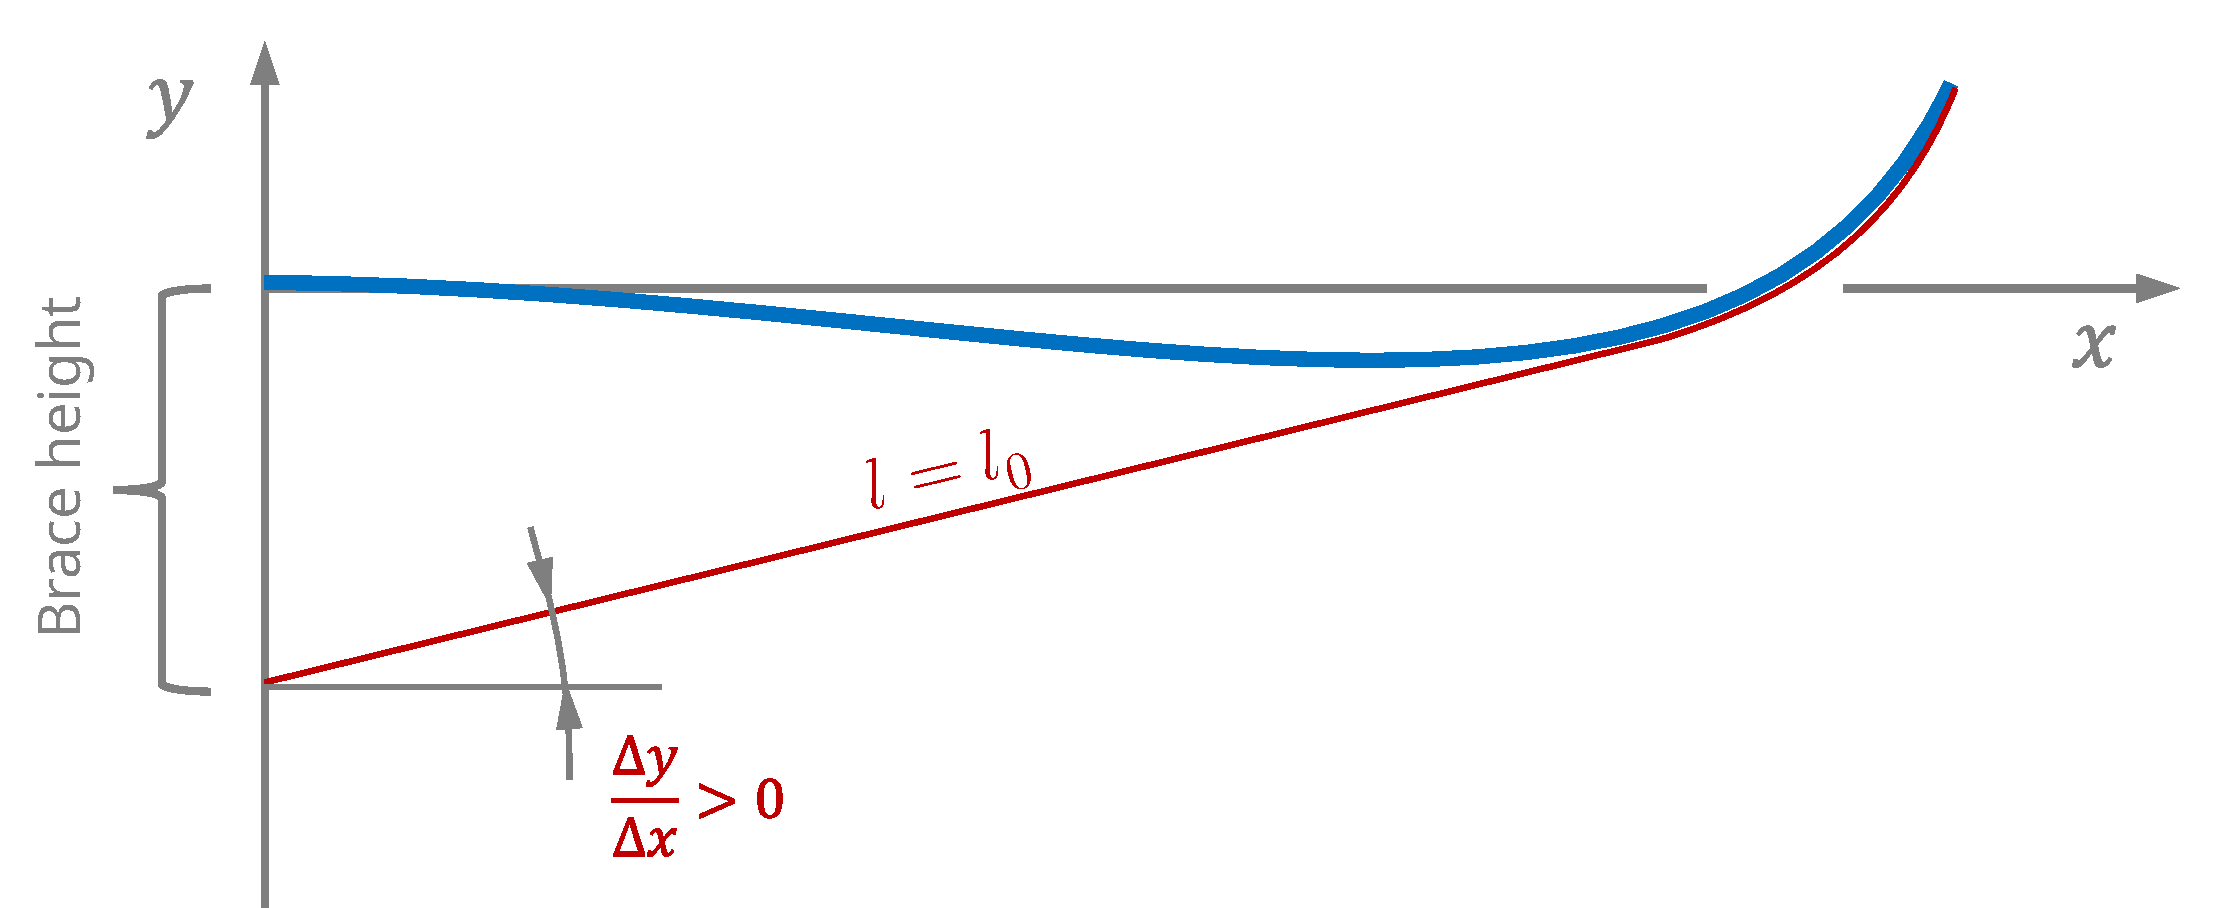
\includegraphics[width=0.7\textwidth]{figures/solution/bracing-method-1}
\caption{Unbraced state}
\label{fig:bracing-method-1}
\end{figure}

At the point where the string intersects the $y$ axis, it initially has a positive slope of $\Delta y / \Delta x$ as measured against the $x$ direction.
If this initial slope were negative, the bow model would have to be rejected as invalid because the specified brace height is too low for the given limb geometry.
The actual bracing process now consists of successively shortening the string (and iterating for equilibrium each time) until the slope reaches zero, while keeping the string center pinned at the desired brace height via displacement control.
This pinning of the string ensures a favorable angle (not too shallow) between string and limb.

\begin{figure}[h]
\centering
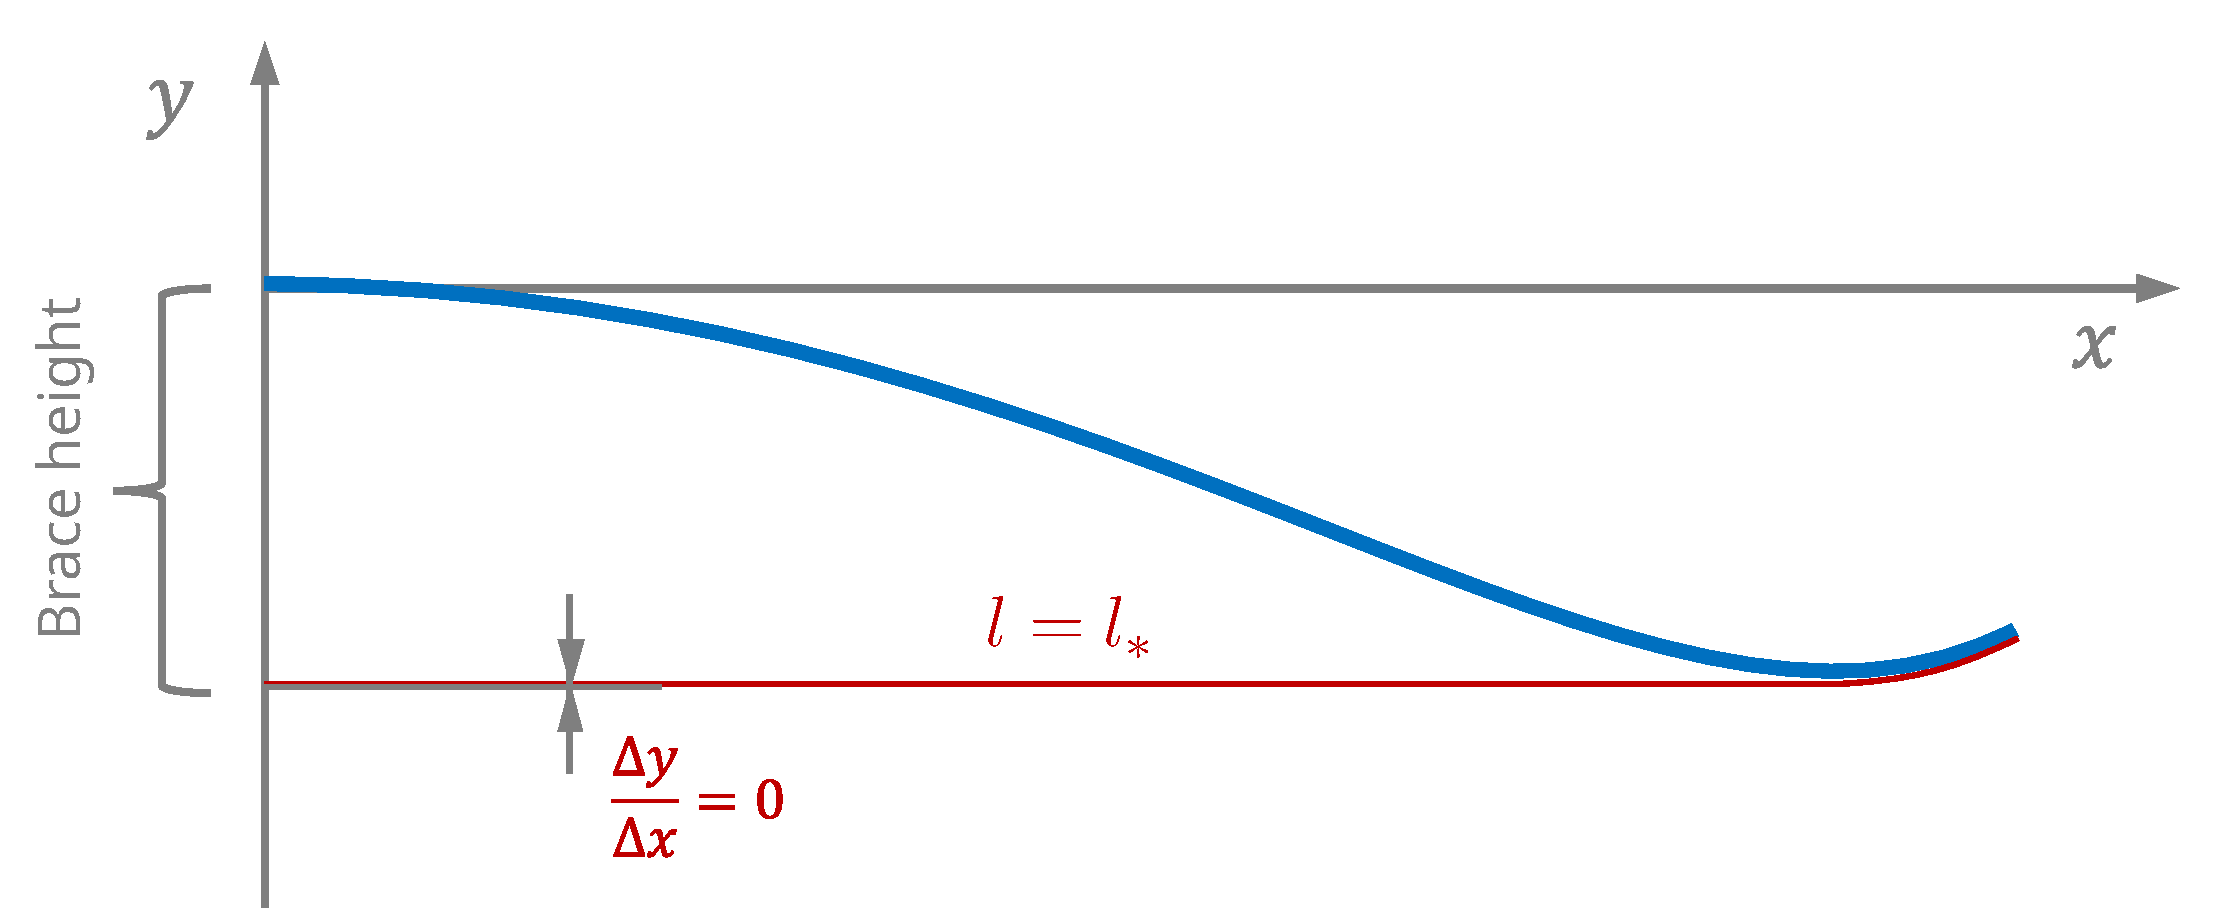
\includegraphics[width=0.7\textwidth]{figures/solution/bracing-method-2}
\caption{Braced state}
\label{fig:bracing-method-2}
\end{figure}

As the string becomes shorter, the slope decreases until it crosses into the negative.
The final string length $l_*$ is the length for which the slope is approximately zero.
This is shown in figure \ref{fig:bracing-method-2}.
So it all reduces to the problem of finding the root $\frac{\Delta y}{\Delta x}(l) = 0$ of the slope as a function of the string length.
This can be made dimensionless by introducing the length reduction factor $p = \frac{l}{l_{0}}$ and writing the slope as $\frac{\Delta y}{\Delta x}(p)$ instead.
Figure \ref{fig:bracing-plot} shows that relationship for a real example, where the final string length is found to be approximately~$0.96\,l_{0}$.

\begin{figure}[h]
\centering
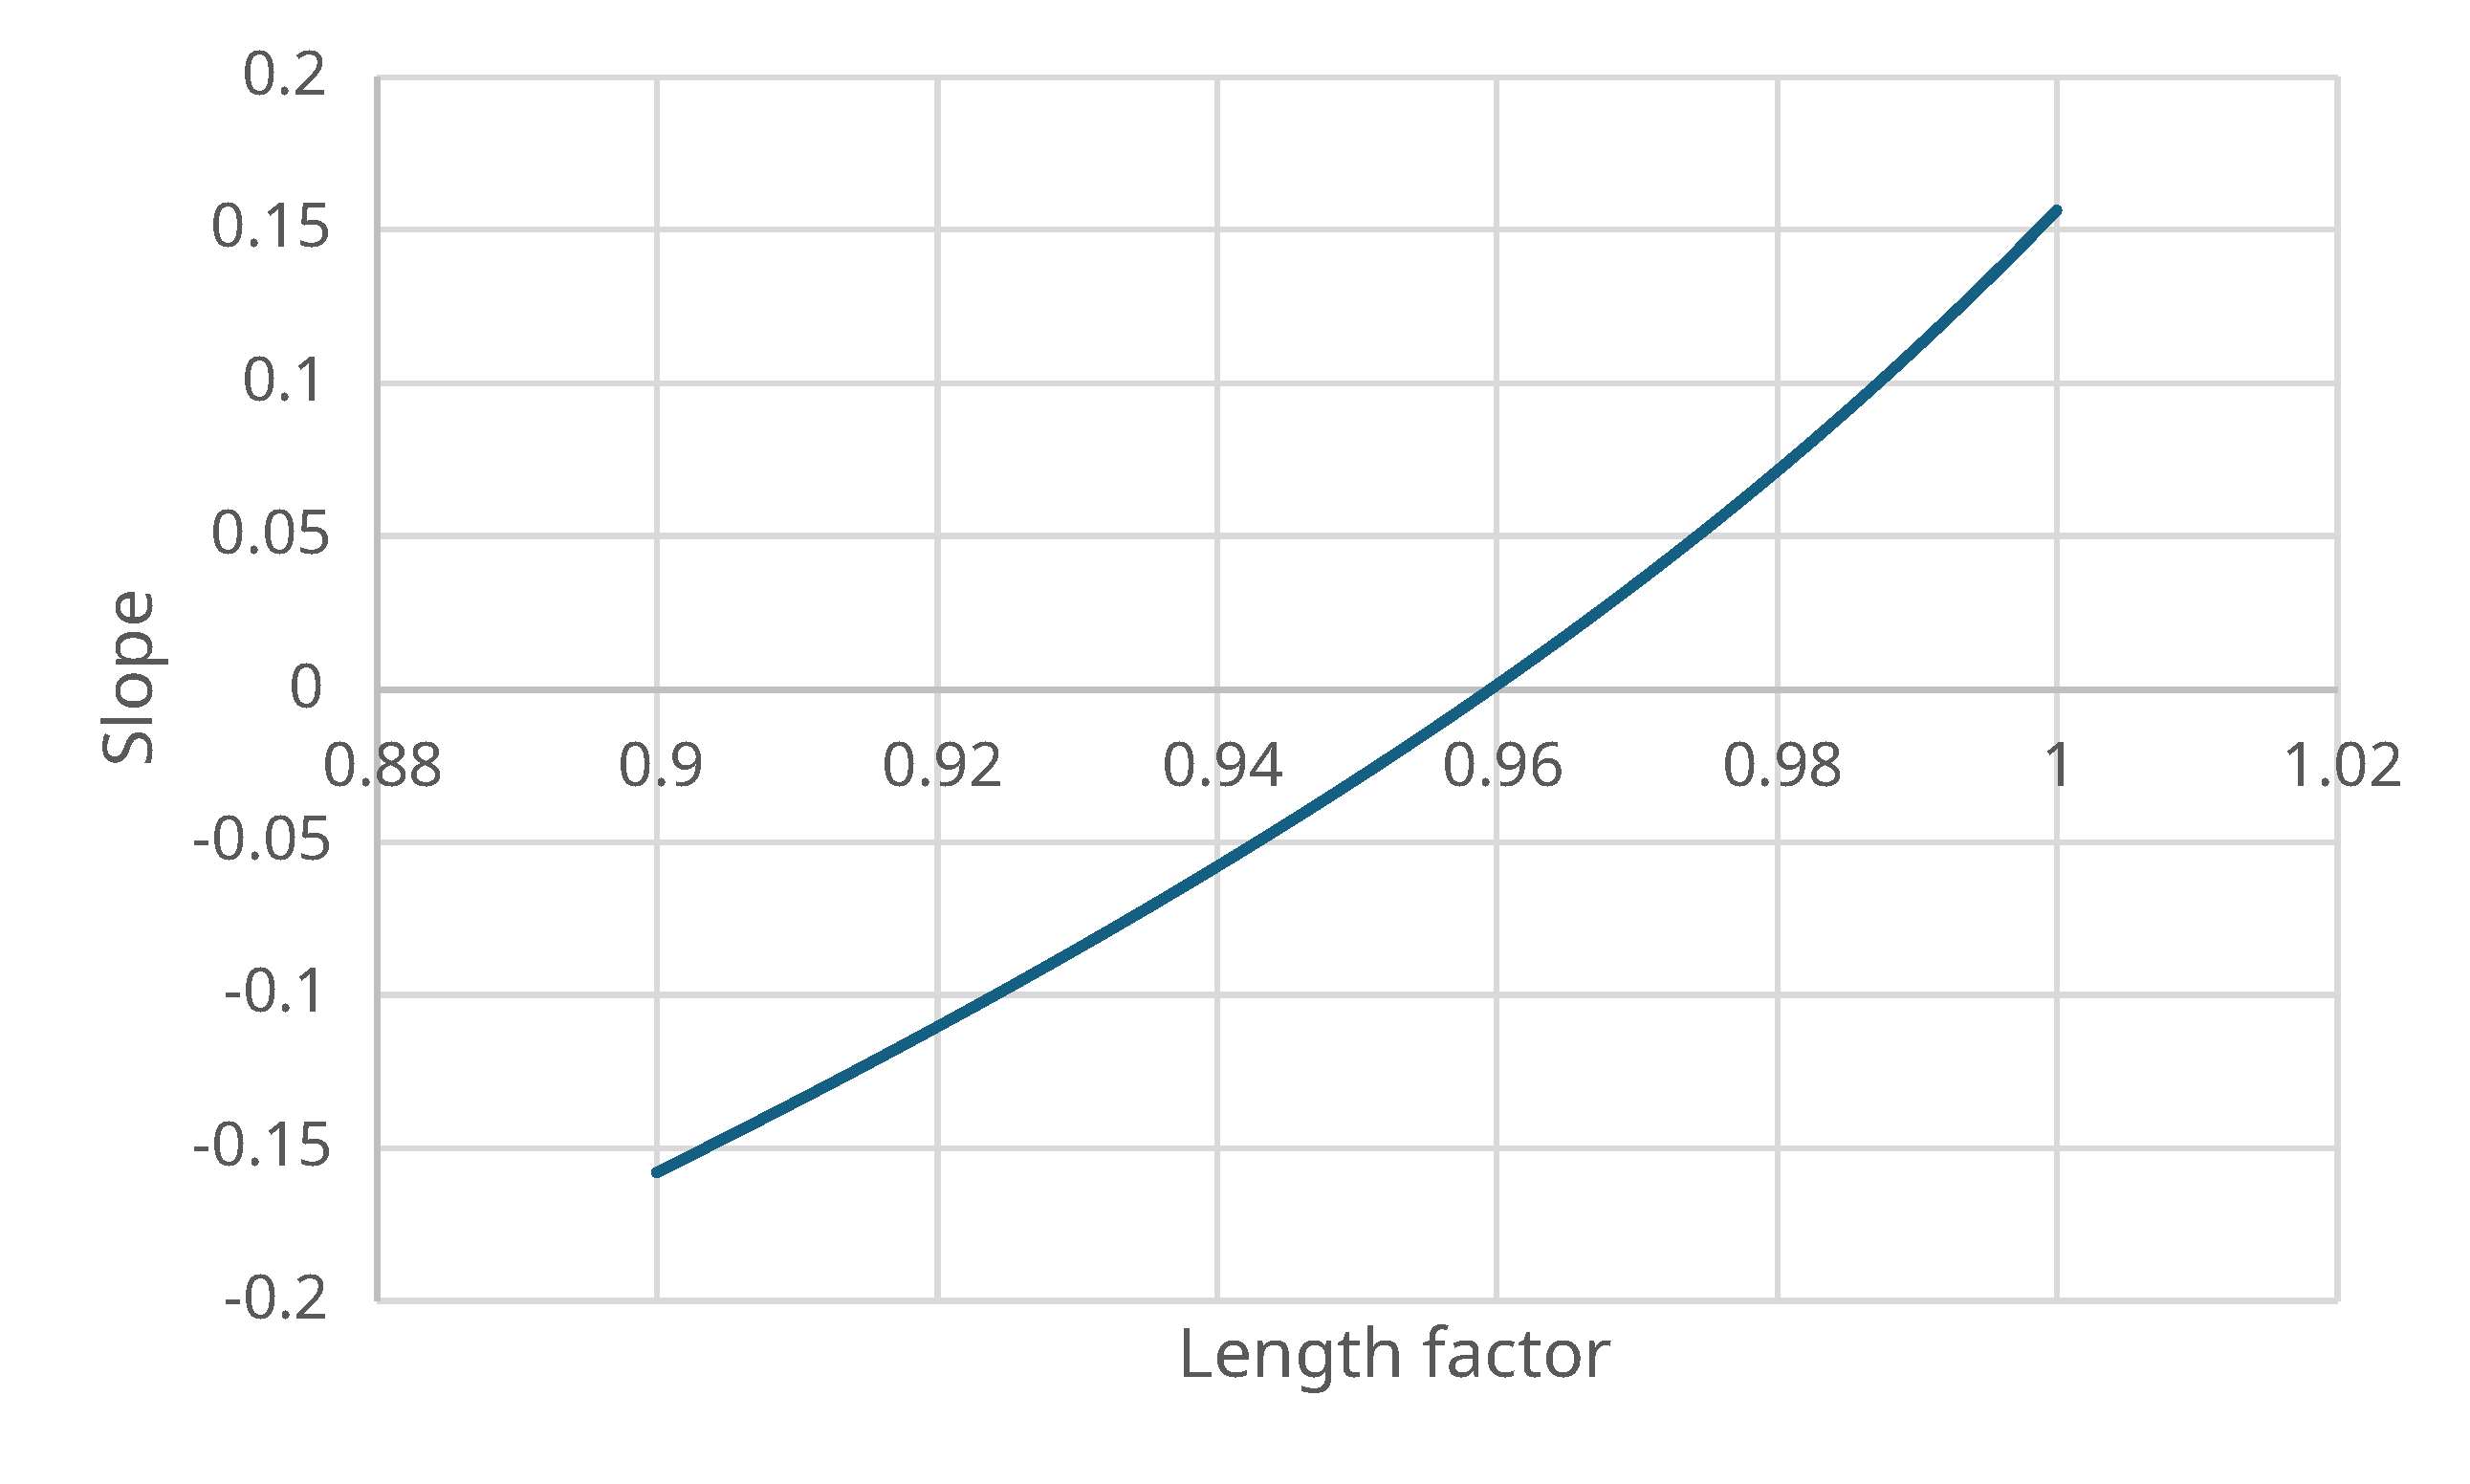
\includegraphics[width=0.6\textwidth]{figures/solution/bracing-plot}
\caption{Slope over string length for a real example}
\label{fig:bracing-plot}
\end{figure}

However, if we just use one of the many standard root finding algorithms for this, it might make big steps in string length and cause the underlying static equilibrium iteration to fail.
Instead, the method starts at $p = 1$ and treats the problem like finding an equilibrium path with the path parameter $p$.
This parameter is controlled just as described in the previous section, taking into account maximum and minumum bounds on the step size and the performance of the static iterations.
A dedicated root finding algorithm is only used after the first negative slope is encountered in order to hone in on a precise final result.
Currently this is the regula falsi method, which is simple and reasonably effective when derivatives are not available and the interval in which the root lies is known.